\section{Creating a local repository\label{sec:local_repo}}

This section covers the following:

\begin{enumerate}
	\item Registering a GitHub username
	\item Download git software
	\item Fork the master repository
\end{enumerate}

\subsection{Git username and profile}

The first step is to create a username and profile on GitHub (if you do not already have one). Creating a username and profile on GitHub is free and easy to do. 

Go to \url{https://www.github.com} to register a username and set up a profile if you do not already have one. See the help at GitHub for more information. Once you have set up a GitHub account, you need to download the git software (see next section) so you can push and pull changes between your local repository and the main online repository.

\subsection{Git software}

You will need to acquire a git client in order to clone the repository to your local machine.

\CNAME\ also requires a command line version of git in order to compile. The \CNAME\ build environment requires \texttt{git} in order to evaluate the version of the code used at compile time to include into the executable, manuals, etc. when being built. 

You will need to download the git client from \href{https://git-scm.com/downloads}{git software} and you will need to make sure that it has been included into your system path. This can be checked by opening a terminal (powershell or command prompt and typing in \texttt{git -v}. Git is a command line program, you can also download a GUI interface which helps using git a lot more user-friendly. My personal preference is the \href{https://desktop.github.com/}{github desktop application}. 

\subsection{Cloning a repository}

The publicly available \CNAME\ code is in the master repository. Only the \CNAME\ Development Team have permission to add, delete, or change code directly to the master repository. 

To clone the master repository, navigate to \url{https://github.com/NIWAFisheriesModelling/CASAL2} and use the green code button, which is shown below to clone. There are multiple protocols (https, ssh etc.) for cloning highlighted in the red box. We recommend using the GitHub desktop method which is circled in Figure~\ref{fig:clone}.

\begin{figure}[H]
	\centering
	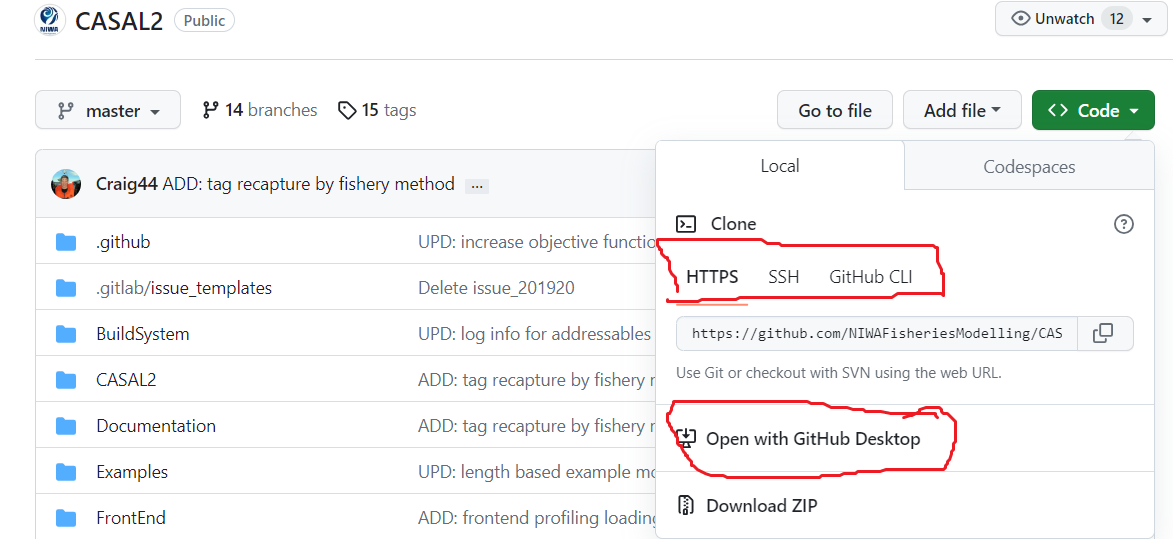
\includegraphics[scale=0.6]{Figures/clone_repo.png}
	\caption{Cloning a repository}\label{fig:clone}
\end{figure}


\subsection{Adding an SSH authentication key to your account on GitHub.com}

One of the reasons contributors may have difficulty pushing and pulling changes to \CNAME\ is because they don't have a SSH authentication key linked to their GitHub account. The error message may look like that shown in Figure~\ref{fig:permissiondenied}. Please see the information from \href{https://docs.github.com/en/authentication/connecting-to-github-with-ssh/adding-a-new-ssh-key-to-your-github-account}{this link} for detailed instructions on how to create a public SSH key on your computer and then link it to your GitHub account.

\begin{figure}[H]
	\centering
	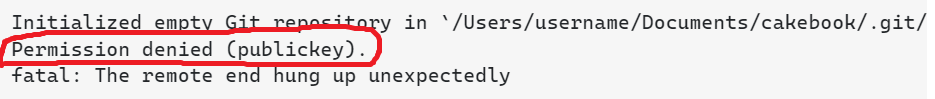
\includegraphics[scale=0.6]{Figures/permissiondenied.png}
	\caption{Example of the error message when SSH authentication has not been enabled}\label{fig:permissiondenied}
\end{figure}
